\documentclass[conference]{IEEEtran}
\usepackage{graphicx}
\usepackage{amssymb}
\usepackage{epstopdf}
% \begin{figure}[h]
%     \centering
%     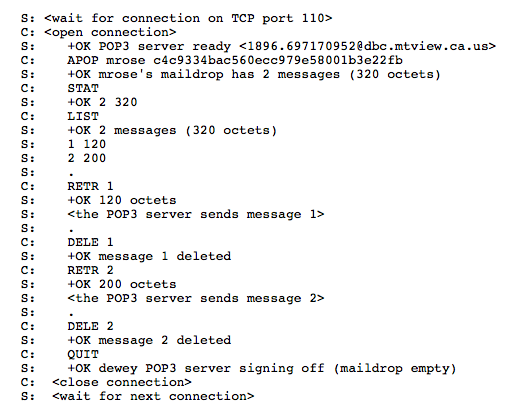
\includegraphics[scale=0.25]{images/pop3.png}
%     \caption{Ancient horrors manifesting through the POP3 protocol.}
%     \label{fig:how_pop3_works}
% \end{figure}
\usepackage[table]{xcolor}
\usepackage{xcolor}
\usepackage{url}
\usepackage{listings}
\usepackage{supertabular, booktabs}
\newcommand{\tech}[1]{\textcolor{green}{#1}}
\newcommand{\acronym}[1]{\textcolor{blue}{#1}}
\newcommand{\ask}[2]{\textcolor{red}{#1}(\textcolor{purple}{#2})}
\DeclareGraphicsRule{.tif}{png}{.png}{`convert #1 `dirname #1`/`basename #1
.tif`.png}

\begin{document}
\title{Studio di un \textit{Time Series Database} in un contesto applicativo reale}

\author{\IEEEauthorblockN{Dr.~Giovanni Cavallin}
\IEEEauthorblockA{Dip. di Matematica\\
Università degli Studi di Padova\\
Email: giovanni.cavallin.1@studenti.unipd.it}}

\maketitle

\begin{abstract}
    briefly describe your problem, approach, and key results (no more than 300 words)
\end{abstract}

\section{Introduzione}
Introduzione alla realtà aziendale in cui il mio progetto si pone, mettendo in evidenza le attuali criticità che hanno portato all'analisi di nuove piattaforme da proporre.

\begin{table}[!ht]
    \begin{center}
        \caption{Alcune tabelle ordinate per dimensione}
        \label{tab:dim_ordered_tables}
        \rowcolors{2}{gray!25}{white}
        \begin{tabular}{l|l}
            \rowcolor{gray!50}
            \textbf{Nome tabella} & \textbf{Dimensione (MB)} \\
            \hline
            TrendTimeSlotHour & 39667.92\\
            TrendTAInst & 37575.00\\
            TrendTimeSlotSmartInfo & 25276.00\\
            TrendTAHour & 19270.95\\
            TrendWMeterInst & 16196.00\\
            TrendTAEnergyHour & 11697.28\\
            TrendPlant & 8537.20\\
            TrendRefHour & 4989.47\\
            TrendWMeterHour & 4896.97\\
            ... & ...\\
            \hline
        \end{tabular}
    \end{center}
\end{table}
\cite{ms_excel}

\paragraph{Estrazione dei dati mancanti}
data la mancanza dell'energia prodotta, consumata e quindi venduta e acquistata, si è dovuto provvedere al suo calcolo. L'energia è calcolabile attraverso la potenza \(P\) e l'intervallo di tempo \(\delta T\) secondo la formula: 
\(E = P\times \delta T \)
La potenza invece, essendo i sistemi mono, bi e trifase e attiva e reattiva, è stata calcolata con:
$\ P = \sqrt{\sum_{f=1}^{3} P_f^{2} + \sum_{f=1}^{3} Q_f^{2}}$
dette \(P_f\) e \(Q_f\) rispettivamente la potenza attiva e reattiva.

\begin{figure}[!ht]
    \centering
    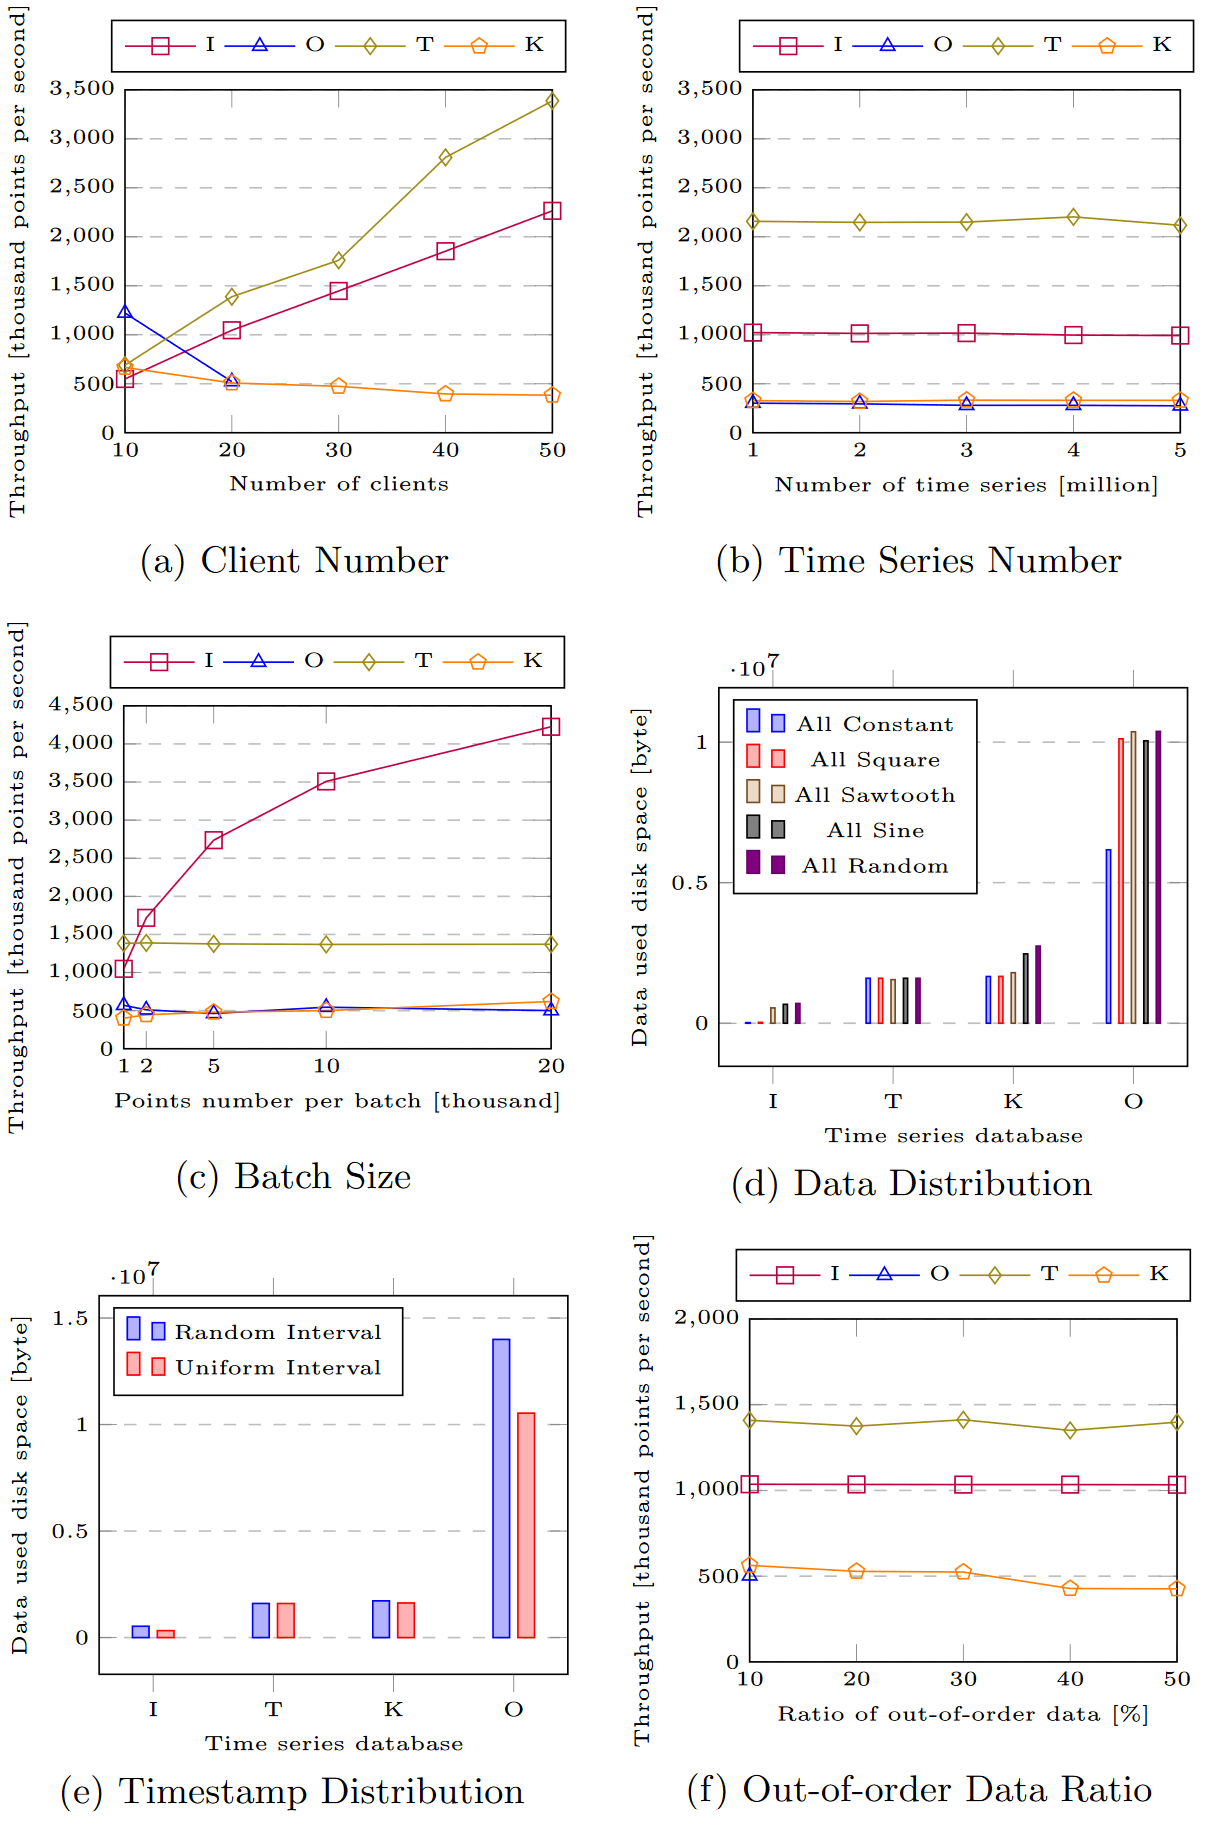
\includegraphics[scale=0.34]{images/data_ingestion_benchmark.png}
    \caption{Esperimenti di ingestione di dati. I, T, K e O individuano InfluxDB, TimescaleDB, KairosDB e OpenTSDB.}
    \label{tab:data_ingestion_benchmark}
\end{figure}

%%%%%%%%%%%%%%%%%%%%%%%%%%%%%%%%%%%%%%%%%%%%%%%%%%%%%%%%%%%%%%%%%%%%%%%%%%%%%%%%%%%%%%%%%%%%%%%%%%%%



\section{Progetti correlati}

\section{Valutazione}

\section{Conclusioni}

\nocite{*} % Include everything in the .bib file.

\bibliographystyle{IEEEtran}
\bibliography{paper}

% that's all, folks
\end{document}
